\subsection{DISP and SIGN}
\label{energy}

The performance of the models trained with the previously mentioned setup,
can be gauged looking at 
figure \ref{fig:disp_perf}. For the DISP regressor model,
the R$^2$ score is chosen as a measure for performance. 
In the case of the SIGN classification model, it is the accuracy.
Both models perform better for higher event energies with accuracy and
R$^2$ reaching values close to 1.
At low energies the results do not seem to match the general trend.
Because the bins are chosen to be of equal width, they do not contain
comparable event counts especially at the lowest and highest energies.
This in combination with different telescopes triggering at different
energies explains the behaviour at those energies.
% For a plot with equally filled bins (of different width) have a look
% at the appendix \ref{app:plots}.

\begin{figure}
    \centering
    \captionsetup{width=0.9\linewidth}
    \begin{subfigure}{0.45\textwidth}
        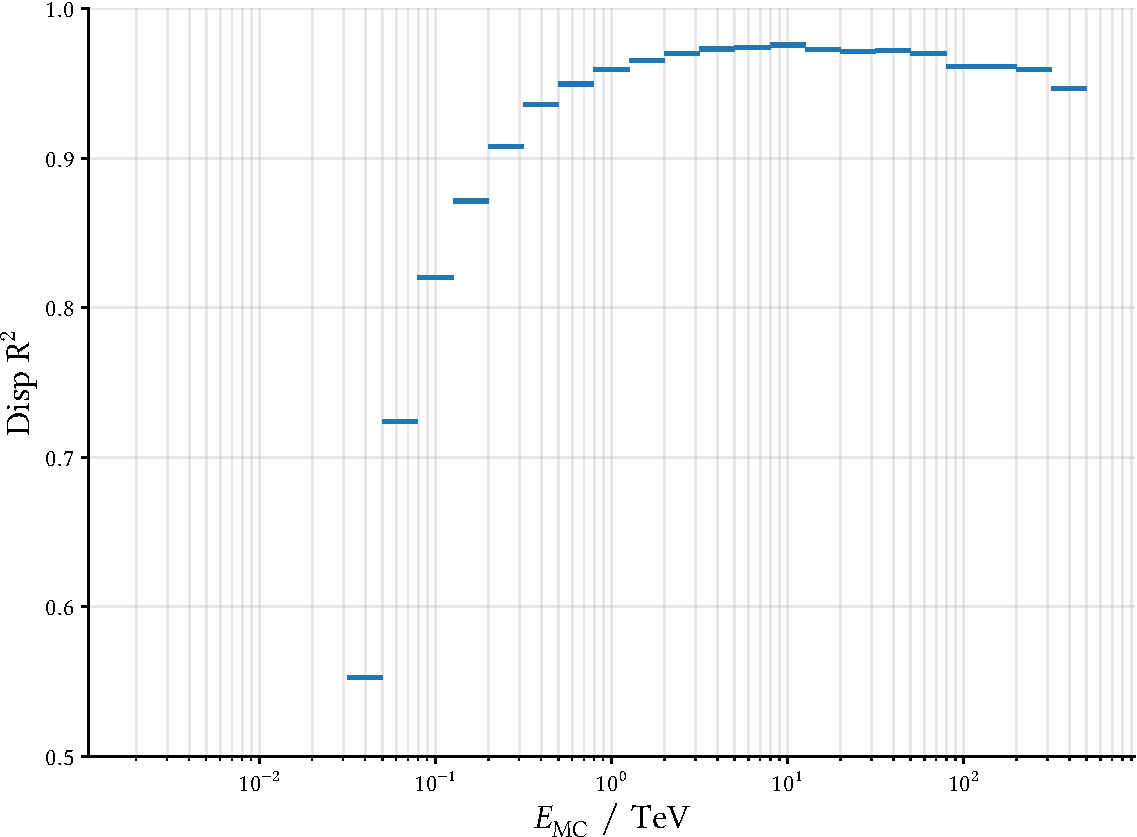
\includegraphics[width=\linewidth]{../analysis/plots/disp_gamma_r2_equal_sized.pdf} 
        \caption{R2-Score for the DISP-estimation}
    \end{subfigure}
    \begin{subfigure}{0.45\textwidth}
        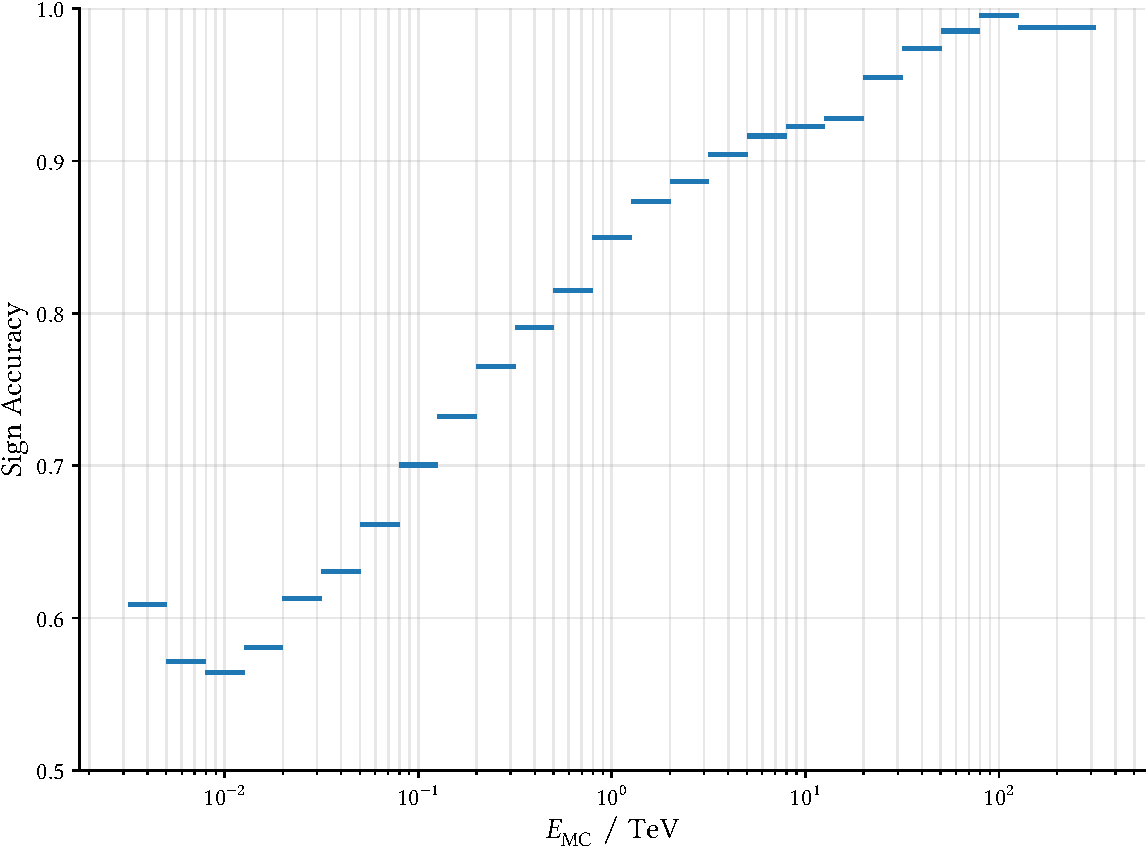
\includegraphics[width=\linewidth]{../analysis/plots/disp_gamma_acc_equal_sized.pdf}
        \caption{Accuracy for the SIGN-estimation}
    \end{subfigure}
    \caption{Performance of the DISP and SIGN model on the cross validated training
    data. In general both models performances improve with increasing energies.}
    % At low energies signs of overfitting can be noticed.}
    \label{fig:disp_perf}
\end{figure}

The feature importances are illustrated in the figures \ref{fig:disp_features}
for the DISP and \ref{fig:sign_features} for the SIGN model.
For the DISP model the stereoscopic features provide the most information.
Besides that, the light content, concentration and the length of the ellipse
are of most importance. Some separation into the different telescope types
seems to happen as well.
In the case of the SIGN model on the other hand, the predictions are almost
entirely based on the $skewness$ and $slope$ of the image.
The stereoscopic features do not provide much information in this case.
% which is expected as the head-/tail-ambiguation is entirely an artefact produced
% in the camera frame.

\begin{figure}
	\centering
    \captionsetup{width=0.9\linewidth}
	\hspace*{-0.11\textwidth}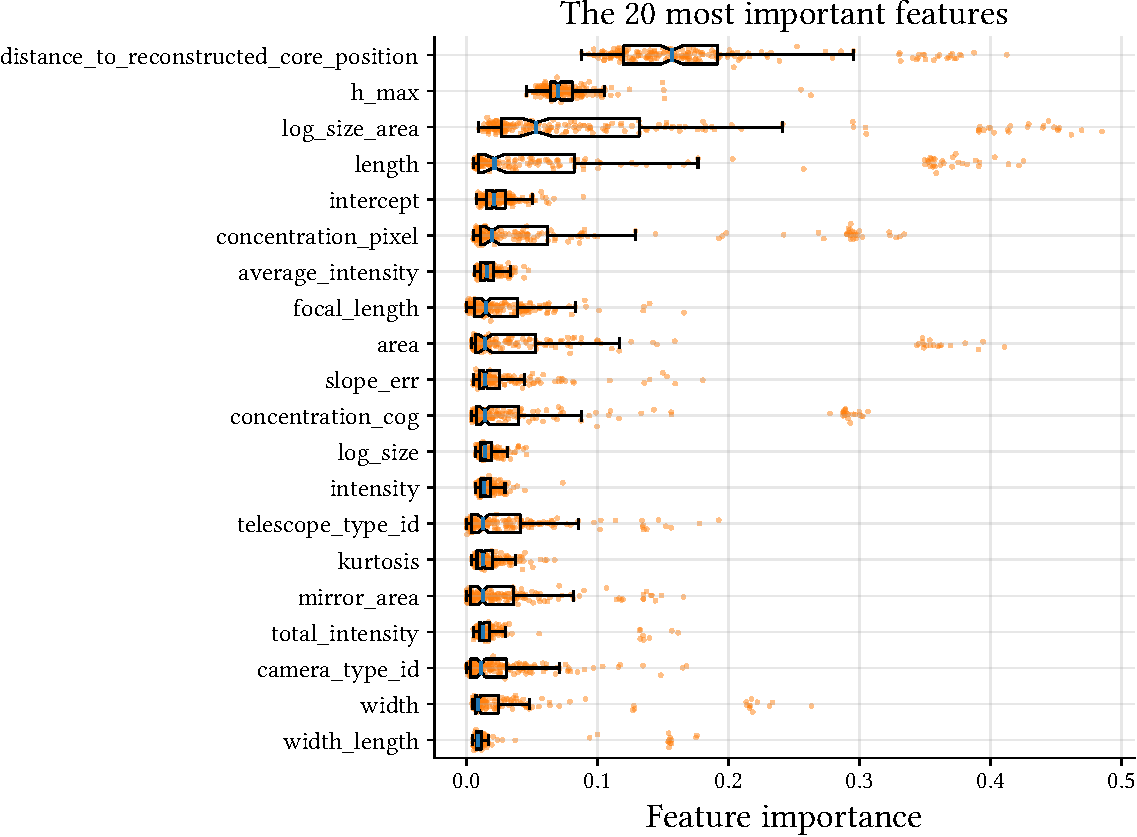
\includegraphics[width=0.6\textwidth]{../analysis/plots/disp_features.pdf}
	\caption{
	    Feature importance of the random forest for the DISP model.
	    The stereoscopic features have high influence on the prediction.
    	From the monoscopic features, the features describing the light content and the
        shape of the ellipse, provide most information.
        Additionaly the $concentration$-features, the $area$, $width$ and $length$
        are of high importance to the model.}
	\label{fig:disp_features}
\end{figure}

\begin{figure}
	\centering
    \captionsetup{width=0.9\linewidth}
	\hspace*{-0.1\textwidth}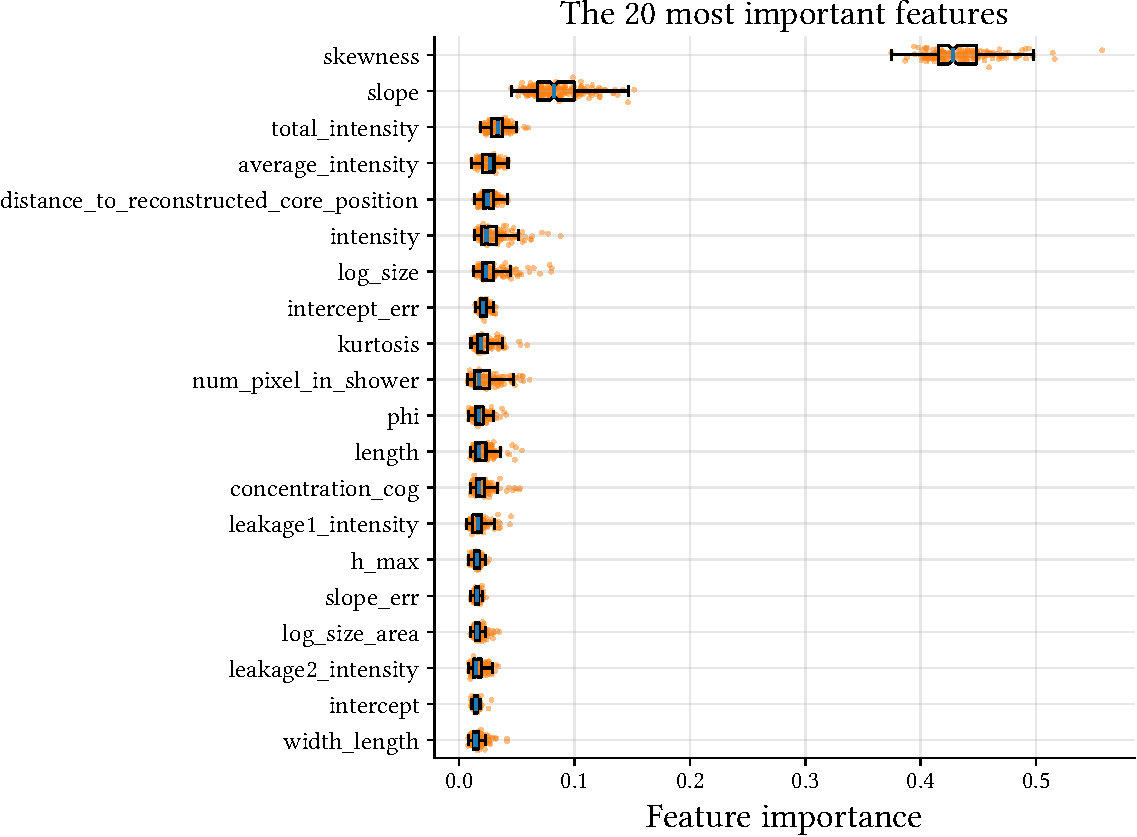
\includegraphics[width=0.6\textwidth]{../analysis/plots/sign_features.pdf}
	\caption{Feature importance of the random forest for the SIGN model.
	        The most influential features to the prediction are by far the higher-order moments $skewness$
            and $slope$. Other features provide very little information.}
	\label{fig:sign_features}
\end{figure}

